%****************************************************************************************************************************************
% File: cps-ontology.tex
%
% This file is automatically generated. Please do not edit!
%****************************************************************************************************************************************
\section{Ontology Overview}

\todoAuthors{Provide ``rdfs:comment'' annotation in ontology}

Figure \ref{fig:cps_ontology_overview} shows an overview of the CPS ontology. The details of each concept are
provided in the following subsections.

\begin{figure}[!htb]
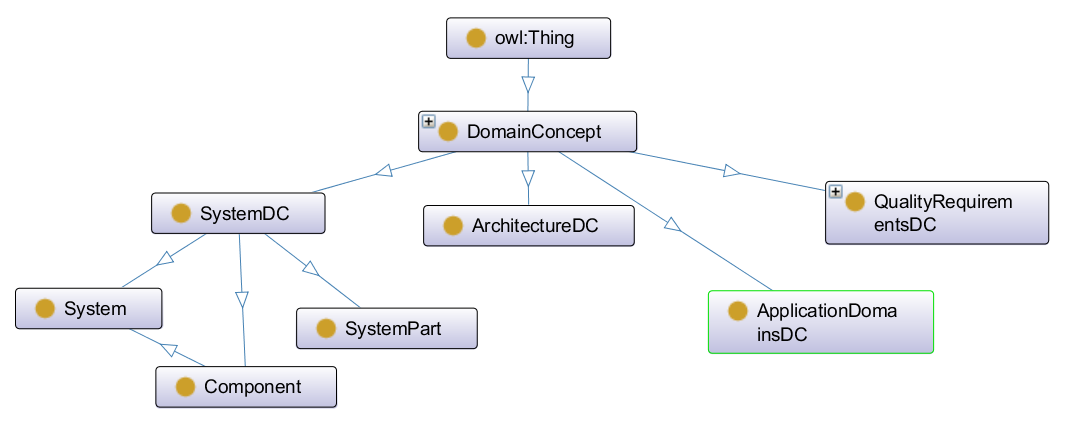
\includegraphics[width=\textwidth]{figures/cps_ontology_overview.png}
\caption{Overview of the CPS ontology}
\label{fig:cps_ontology_overview}
\end{figure}
	
\section{Domain Concepts}
\label{sec:cps:classes}

This ontology of cyber-physical systems contains concepts divided into sub-domains as presented in the following subsections.

\subsection{CPSDC}
\label{subsecDC:CPSDC}

\todoAuthors{Provide ``rdfs:comment'' annotation in ontology}

\subsubsection{Action}
\label{subsubsecC:Action}
\didx{Action}

Humans within a CPS exercise their responsibilities defined by roles by performing certain actions. Action is an entity that is targeted at changing the state of the CPS or environment. Actions are divided into physical actions, communicative actions, and epistemic actions.

\textbf{Subclass of}
\begin{itemize}
	\item \textbf{CPSDC} (see section \ref{subsecDC:CPSDC})
	\item \textbf{Action} (see section \ref{subsubsecC:Action})
\end{itemize}






\subsubsection{Actuator}
\label{subsubsecC:Actuator}
\didx{Actuator}

External devices or components of the system which act on parts of the system to modify its behaviour.

\textbf{Subclass of}
\begin{itemize}
	\item \textbf{Physical} (see section \ref{subsubsecC:Physical})
\end{itemize}






\subsubsection{Application-specificCircuit}
\label{subsubsecC:Application-specificCircuit}
\didx{Application-specificCircuit}

Application-specific circuits are various additional circuit-based components that are connected to the controller. It includes all kinds of bespoke circuits that are not processor, memory or interfaces, for example, hardware accelerators, signal processors, etc.

\textbf{Subclass of}
\begin{itemize}
	\item \textbf{CPSDC} (see section \ref{subsecDC:CPSDC})
\end{itemize}






\subsubsection{ApplicationDomain}
\label{subsubsecC:ApplicationDomain}
\didx{ApplicationDomain}

This class describes the various domains and industrial sectors which the cyber-physical system is concerned with.

\textbf{Subclass of}
\begin{itemize}
	\item \textbf{CPSDC} (see section \ref{subsecDC:CPSDC})
\end{itemize}






\subsubsection{ApplicationLayer}
\label{subsubsecC:ApplicationLayer}
\didx{ApplicationLayer}

The application layer orchestrates the services to provide emergent properties.

\textbf{Subclass of}
\begin{itemize}
	\item \textbf{CPSDC} (see section \ref{subsecDC:CPSDC})
\end{itemize}






\subsubsection{ApplicationSoftware}
\label{subsubsecC:ApplicationSoftware}
\didx{ApplicationSoftware}

Application software (app for short) is a program or group of programs designed for end users. Application software is built for specific tasks. While system software programs run in the background, application software runs in the foreground and users interact with it. System software programs work on its own while application software is dependent on it.

\textbf{Subclass of}
\begin{itemize}
	\item \textbf{Software} (see section \ref{subsubsecC:Software})
\end{itemize}






\subsubsection{Architecture}
\label{subsubsecC:Architecture}
\didx{Architecture}

\todoAuthors{Provide ``rdfs:comment'' annotation in ontology}

\textbf{Subclass of}
\begin{itemize}
	\item \textbf{Architecture} (see section \ref{subsubsecC:Architecture})
	\item \textbf{CPSDC} (see section \ref{subsecDC:CPSDC})
	\item \textbf{ArchitectureDC} (see section \ref{subsecDC:ArchitectureDC})
\end{itemize}






\subsubsection{Architecture}
\label{subsubsecC:Architecture}
\didx{Architecture}

\todoAuthors{Provide ``rdfs:comment'' annotation in ontology}

\textbf{Subclass of}
\begin{itemize}
	\item \textbf{Architecture} (see section \ref{subsubsecC:Architecture})
	\item \textbf{CPSDC} (see section \ref{subsecDC:CPSDC})
	\item \textbf{ArchitectureDC} (see section \ref{subsecDC:ArchitectureDC})
\end{itemize}






\subsubsection{AuxiliaryMemory}
\label{subsubsecC:AuxiliaryMemory}
\didx{AuxiliaryMemory}

Devices that provide backup storage are called auxiliary memory. It is not directly accessible to the CPU, and is accessed using the Input/Output channels. Magnetic disks and tapes are commonly used auxiliary devices. Other devices used as auxiliary memory are magnetic drums, magnetic bubble memory and optical disks.

\textbf{Subclass of}
\begin{itemize}
	\item \textbf{Memory} (see section \ref{subsubsecC:Memory})
\end{itemize}






\subsubsection{Behavior}
\label{subsubsecC:Behavior}
\didx{Behavior}

Dynamical pattern.

\textbf{Subclass of}
\begin{itemize}
	\item \textbf{CPSDC} (see section \ref{subsecDC:CPSDC})
	\item \textbf{Behavior} (see section \ref{subsubsecC:Behavior})
\end{itemize}






\subsubsection{CPS}
\label{subsubsecC:CPS}
\didx{CPS}

The top-level class that encapsulates cyber-physical systems.

\textbf{Subclass of}
\begin{itemize}
	\item \textbf{CPS} (see section \ref{subsubsecC:CPS})
	\item \textbf{CPSDC} (see section \ref{subsecDC:CPSDC})
\end{itemize}






\subsubsection{CPSComponentLayer}
\label{subsubsecC:CPSComponentLayer}
\didx{CPSComponentLayer}


	The CPS component layer includes the capabilities for the CPS
	components to undertake sensing and actuation.


\textbf{Subclass of}
\begin{itemize}
	\item \textbf{CPSDC} (see section \ref{subsecDC:CPSDC})
\end{itemize}






\subsubsection{ComType}
\label{subsubsecC:ComType}
\didx{ComType}

The class models the type of communication: whether it is synchronus or asynchronous.

\textbf{Subclass of}
\begin{itemize}
	\item \textbf{CPSDC} (see section \ref{subsecDC:CPSDC})
\end{itemize}






\subsubsection{Communication}
\label{subsubsecC:Communication}
\didx{Communication}

This class models the communication system and the communication protocols used in the network between the different components of the cyber-physical system.

\textbf{Subclass of}
\begin{itemize}
	\item \textbf{Communication} (see section \ref{subsubsecC:Communication})
	\item \textbf{CPSDC} (see section \ref{subsecDC:CPSDC})
\end{itemize}






\subsubsection{CommunicationAction}
\label{subsubsecC:CommunicationAction}
\didx{CommunicationAction}

A communicative action is a kind of action that sends a message through a communication network of the CPS.

\textbf{Subclass of}
\begin{itemize}
	\item \textbf{Action} (see section \ref{subsubsecC:Action})
\end{itemize}






\subsubsection{Configuration}
\label{subsubsecC:Configuration}
\didx{Configuration}

Network configuration is also known as network topology. This class describes how the nodes/devices/components in the system network are arranged and how they communicate with each other.

\textbf{Subclass of}
\begin{itemize}
	\item \textbf{CPSDC} (see section \ref{subsecDC:CPSDC})
\end{itemize}






\subsubsection{ConstituentElement}
\label{subsubsecC:ConstituentElement}
\didx{ConstituentElement}

The class that encompasses all the different elements that actually constitute the cyber-physical system.

\textbf{Subclass of}
\begin{itemize}
	\item \textbf{CPSDC} (see section \ref{subsecDC:CPSDC})
	\item \textbf{ConstituentElement} (see section \ref{subsubsecC:ConstituentElement})
\end{itemize}






\subsubsection{Constraints}
\label{subsubsecC:Constraints}
\didx{Constraints}

Constraints are conditions that a human performing the role must take into consideration when exercising its responsibilities.

\textbf{Subclass of}
\begin{itemize}
	\item \textbf{CPSDC} (see section \ref{subsecDC:CPSDC})
\end{itemize}






\subsubsection{Continuity}
\label{subsubsecC:Continuity}
\didx{Continuity}

This class describes the property of the state of the system and how it's graph (versus time) behaves in terms of continuity. Whether it is continuous or discontinuous.

\textbf{Subclass of}
\begin{itemize}
	\item \textbf{CPSDC} (see section \ref{subsecDC:CPSDC})
\end{itemize}






\subsubsection{Control}
\label{subsubsecC:Control}
\didx{Control}

The action of modifying the behaviour of a system through feedback.

\textbf{Subclass of}
\begin{itemize}
	\item \textbf{Control} (see section \ref{subsubsecC:Control})
	\item \textbf{ConstituentElement} (see section \ref{subsubsecC:ConstituentElement})
\end{itemize}






\subsubsection{Controller}
\label{subsubsecC:Controller}
\didx{Controller}

External device or component of the system which produces the control signal to modify the system behaviour.

\textbf{Subclass of}
\begin{itemize}
	\item \textbf{Physical} (see section \ref{subsubsecC:Physical})
\end{itemize}






\subsubsection{Cyber}
\label{subsubsecC:Cyber}
\didx{Cyber}

Communication and control between any human/biological/social system and any artificial device. It refers to systems where feedback is essential.

\textbf{Subclass of}
\begin{itemize}
	\item \textbf{Cyber} (see section \ref{subsubsecC:Cyber})
	\item \textbf{ConstituentElement} (see section \ref{subsubsecC:ConstituentElement})
\end{itemize}






\subsubsection{Dependency}
\label{subsubsecC:Dependency}
\didx{Dependency}

This class models the dependencies of the feedback mechanism in the control of the system. The feedback loop can be a function of the state and/or the output of the system.

\textbf{Subclass of}
\begin{itemize}
	\item \textbf{CPSDC} (see section \ref{subsecDC:CPSDC})
\end{itemize}






\subsubsection{Diagnostics}
\label{subsubsecC:Diagnostics}
\didx{Diagnostics}

Identification of properties in a system.

\textbf{Subclass of}
\begin{itemize}
	\item \textbf{CPSDC} (see section \ref{subsecDC:CPSDC})
\end{itemize}






\subsubsection{Disciplines}
\label{subsubsecC:Disciplines}
\didx{Disciplines}

This class describes the various engineering and other disciplines that are associated with the development and application of the cyber-physical system.

\textbf{Subclass of}
\begin{itemize}
	\item \textbf{CPSDC} (see section \ref{subsecDC:CPSDC})
\end{itemize}






\subsubsection{Discontinuous}
\label{subsubsecC:Discontinuous}
\didx{Discontinuous}

Discontinuous or non-smooth systems present some type of discontinuity in the model representing the system. Different names are used depending on the type of discontinuity.

\textbf{Subclass of}
\begin{itemize}
	\item \textbf{Continuity} (see section \ref{subsubsecC:Continuity})
\end{itemize}






\subsubsection{Disturbance}
\label{subsubsecC:Disturbance}
\didx{Disturbance}


						External influence of the environment in a system,
						typically unknown.
					

\textbf{Subclass of}
\begin{itemize}
	\item \textbf{CPSDC} (see section \ref{subsecDC:CPSDC})
\end{itemize}






\subsubsection{Dynamics}
\label{subsubsecC:Dynamics}
\didx{Dynamics}

Evolution of a system over time

\textbf{Subclass of}
\begin{itemize}
	\item \textbf{Dynamics} (see section \ref{subsubsecC:Dynamics})
	\item \textbf{CPSDC} (see section \ref{subsecDC:CPSDC})
\end{itemize}






\subsubsection{Electronic}
\label{subsubsecC:Electronic}
\didx{Electronic}

The execution platform of the control software

\textbf{Subclass of}
\begin{itemize}
	\item \textbf{Electronic} (see section \ref{subsubsecC:Electronic})
	\item \textbf{Controller} (see section \ref{subsubsecC:Controller})
\end{itemize}






\subsubsection{Embedded/FirmwareSoftware}
\label{subsubsecC:Embedded/FirmwareSoftware}
\didx{Embedded/FirmwareSoftware}

Embedded software is computer software, written to control machines or devices that are not typically thought of as computers, commonly known as embedded systems. It is typically specialized for the particular hardware that it runs on and has time and memory constraints. A precise and stable characteristic feature is that no or not all functions of embedded software are initiated/controlled via a human interface, but through machine-interfaces instead. Unlike standard computers that generally use an operating systems such as OS X, Windows or GNU/Linux, embedded software may use no operating system, or when they do use, a wide variety of operating systems can be chosen from, typically a real-time operating system.

\textbf{Subclass of}
\begin{itemize}
	\item \textbf{Software} (see section \ref{subsubsecC:Software})
\end{itemize}






\subsubsection{EmergentBehavior}
\label{subsubsecC:EmergentBehavior}
\didx{EmergentBehavior}

Behaviour that did not exist in the single systems that together form a complex system consisting of interacting systems.

\textbf{Subclass of}
\begin{itemize}
	\item \textbf{Behavior} (see section \ref{subsubsecC:Behavior})
\end{itemize}






\subsubsection{Entity}
\label{subsubsecC:Entity}
\didx{Entity}

An entity is anything perceivable or conceivable (I think that entity should be defined for CPS at a higher level than under human).

\textbf{Subclass of}
\begin{itemize}
	\item \textbf{CPSDC} (see section \ref{subsecDC:CPSDC})
\end{itemize}






\subsubsection{Environment}
\label{subsubsecC:Environment}
\didx{Environment}

What it is not the system.

\textbf{Subclass of}
\begin{itemize}
	\item \textbf{Physical} (see section \ref{subsubsecC:Physical})
\end{itemize}






\subsubsection{EpistemicAction}
\label{subsubsecC:EpistemicAction}
\didx{EpistemicAction}

An epistemic action is a kind of action that changes the state of the data held by the CPS. A human performs actions through actuators.

\textbf{Subclass of}
\begin{itemize}
	\item \textbf{Action} (see section \ref{subsubsecC:Action})
\end{itemize}






\subsubsection{Equilibrium}
\label{subsubsecC:Equilibrium}
\didx{Equilibrium}

States of the system that represent set points.

\textbf{Subclass of}
\begin{itemize}
	\item \textbf{Behavior} (see section \ref{subsubsecC:Behavior})
\end{itemize}






\subsubsection{Event}
\label{subsubsecC:Event}
\didx{Event}

A human can perceive events generated by the CPS or environment. An event is a kind of entity that is related to the states of affairs before and after it has occurred. A human perceives events through sensors.

\textbf{Subclass of}
\begin{itemize}
	\item \textbf{CPSDC} (see section \ref{subsecDC:CPSDC})
\end{itemize}






\subsubsection{ExternalInterfaces}
\label{subsubsecC:ExternalInterfaces}
\didx{ExternalInterfaces}

Interfaces and connections in between componenets of the execution platform.

\textbf{Subclass of}
\begin{itemize}
	\item \textbf{CPSDC} (see section \ref{subsecDC:CPSDC})
\end{itemize}






\subsubsection{Feedback}
\label{subsubsecC:Feedback}
\didx{Feedback}

Implementation of the control action by sensing the output of a system and modifying its input by means of actuators to meet a pre-defined control goal.

\textbf{Subclass of}
\begin{itemize}
	\item \textbf{Feedback} (see section \ref{subsubsecC:Feedback})
	\item \textbf{CPSDC} (see section \ref{subsecDC:CPSDC})
\end{itemize}






\subsubsection{Goal}
\label{subsubsecC:Goal}
\didx{Goal}

Desired behaviour of a system.

\textbf{Subclass of}
\begin{itemize}
	\item \textbf{Goal} (see section \ref{subsubsecC:Goal})
	\item \textbf{CPSDC} (see section \ref{subsecDC:CPSDC})
\end{itemize}






\subsubsection{Human}
\label{subsubsecC:Human}
\didx{Human}

Humans within a CPS perform certain roles within the CPS. 

\textbf{Subclass of}
\begin{itemize}
	\item \textbf{Human} (see section \ref{subsubsecC:Human})
	\item \textbf{ConstituentElement} (see section \ref{subsubsecC:ConstituentElement})
	\item \textbf{Participant} (see section \ref{subsubsecC:Participant})
	\item \textbf{Resource} (see section \ref{subsubsecC:Resource})
\end{itemize}






\subsubsection{Human}
\label{subsubsecC:Human}
\didx{Human}

Humans within a CPS perform certain roles within the CPS. 

\textbf{Subclass of}
\begin{itemize}
	\item \textbf{Human} (see section \ref{subsubsecC:Human})
	\item \textbf{ConstituentElement} (see section \ref{subsubsecC:ConstituentElement})
	\item \textbf{Participant} (see section \ref{subsubsecC:Participant})
	\item \textbf{Resource} (see section \ref{subsubsecC:Resource})
\end{itemize}






\subsubsection{Input}
\label{subsubsecC:Input}
\didx{Input}

Abstraction of the external factors in a system influencing its behaviour.

\textbf{Subclass of}
\begin{itemize}
	\item \textbf{CPSDC} (see section \ref{subsecDC:CPSDC})
\end{itemize}






\subsubsection{Interoperability}
\label{subsubsecC:Interoperability}
\didx{Interoperability}


	The interoperability is the capacity of a product or system whose interfaces are fully known to work with other products or existing or future systems and unrestricted access or implementation.
	Interoperability is different from compatibility. Where compatibility is a vertical notion that a system can operate in agiven environment, interoperability is a transversal notion that allows various systems to communicate and work together.


\textbf{Subclass of}
\begin{itemize}
	\item \textbf{nonfunctionalReqs} (see section \ref{subsubsecC:nonfunctionalReqs})
\end{itemize}






\subsubsection{Linearity}
\label{subsubsecC:Linearity}
\didx{Linearity}

This class describes the property of the system that models the relationship between the input and output. If the transformation relation is linear, the system is classified as linear. If a change in input results in a propotional change in output, the system is linear. If not, the system is lon-linear.

\textbf{Subclass of}
\begin{itemize}
	\item \textbf{CPSDC} (see section \ref{subsecDC:CPSDC})
\end{itemize}






\subsubsection{ManagementLayer}
\label{subsubsecC:ManagementLayer}
\didx{ManagementLayer}

The management layer supports capabilities such as device management, traffic and congestion management.

\textbf{Subclass of}
\begin{itemize}
	\item \textbf{CPSDC} (see section \ref{subsecDC:CPSDC})
\end{itemize}






\subsubsection{Mechanical}
\label{subsubsecC:Mechanical}
\didx{Mechanical}

A mechanical control mechanism like a bi-metallic strip in a thermostat. Its input is made of mechanical effort.

\textbf{Subclass of}
\begin{itemize}
	\item \textbf{Controller} (see section \ref{subsubsecC:Controller})
\end{itemize}






\subsubsection{Memory}
\label{subsubsecC:Memory}
\didx{Memory}

Memory refers to a device that is used to store information for immediate use in a computer or related computer hardware. It typically refers to semi-conductor memory, where data is stored within MOS (Metal-Oxide Semiconductor) cells on an integrated chip.

\textbf{Subclass of}
\begin{itemize}
	\item \textbf{CPSDC} (see section \ref{subsecDC:CPSDC})
\end{itemize}






\subsubsection{Network}
\label{subsubsecC:Network}
\didx{Network}

A set of elements (for example, nodes) connected in some physical or abstract manner (for example, links).

\textbf{Subclass of}
\begin{itemize}
	\item \textbf{Network} (see section \ref{subsubsecC:Network})
	\item \textbf{ConstituentElement} (see section \ref{subsubsecC:ConstituentElement})
\end{itemize}






\subsubsection{NetworkLayer}
\label{subsubsecC:NetworkLayer}
\didx{NetworkLayer}

The network layer provides functionality for networking connectivity and transport capabilities enabling the coordination of components.

\textbf{Subclass of}
\begin{itemize}
	\item \textbf{CPSDC} (see section \ref{subsecDC:CPSDC})
\end{itemize}






\subsubsection{OperatingSystem}
\label{subsubsecC:OperatingSystem}
\didx{OperatingSystem}

An Operating System (OS) is the interface between a user and the hardware of the cyber-physical system. The OS is the software which performs all the basic tasks like management, memory management, process management, handling input and output.

\textbf{Subclass of}
\begin{itemize}
	\item \textbf{OperatingSystem} (see section \ref{subsubsecC:OperatingSystem})
	\item \textbf{SystemSoftware} (see section \ref{subsubsecC:SystemSoftware})
\end{itemize}






\subsubsection{Output}
\label{subsubsecC:Output}
\didx{Output}

Abstraction of the effect of a system on its environment.

\textbf{Subclass of}
\begin{itemize}
	\item \textbf{CPSDC} (see section \ref{subsecDC:CPSDC})
\end{itemize}






\subsubsection{Physical}
\label{subsubsecC:Physical}
\didx{Physical}

This class represents the physical components that constitute the cyber-physical system. 

\textbf{Subclass of}
\begin{itemize}
	\item \textbf{Physical} (see section \ref{subsubsecC:Physical})
	\item \textbf{ConstituentElement} (see section \ref{subsubsecC:ConstituentElement})
\end{itemize}






\subsubsection{PhysicalAction}
\label{subsubsecC:PhysicalAction}
\didx{PhysicalAction}

Physical action is a kind of action that changes the state of a physical element of the CPS or environment.

\textbf{Subclass of}
\begin{itemize}
	\item \textbf{Action} (see section \ref{subsubsecC:Action})
\end{itemize}






\subsubsection{Plant}
\label{subsubsecC:Plant}
\didx{Plant}

System to control.

\textbf{Subclass of}
\begin{itemize}
	\item \textbf{Physical} (see section \ref{subsubsecC:Physical})
\end{itemize}






\subsubsection{Probabilistic}
\label{subsubsecC:Probabilistic}
\didx{Probabilistic}

Probabilistic models incorporate randomness in their approach.

\textbf{Subclass of}
\begin{itemize}
	\item \textbf{Uncertainty} (see section \ref{subsubsecC:Uncertainty})
\end{itemize}






\subsubsection{Processor}
\label{subsubsecC:Processor}
\didx{Processor}

A process or processing unit is a digital circuit which performs operations on some external data source. It typically takes the form of a microprocessor, implented on a metal-oxide semiconductor integrated circuit chip.

\textbf{Subclass of}
\begin{itemize}
	\item \textbf{CPSDC} (see section \ref{subsecDC:CPSDC})
\end{itemize}






\subsubsection{Prognostics}
\label{subsubsecC:Prognostics}
\didx{Prognostics}

Prediction of the time in the future when a system will not performed anymore as it is expected or for what it was designed (control goal).

\textbf{Subclass of}
\begin{itemize}
	\item \textbf{CPSDC} (see section \ref{subsecDC:CPSDC})
\end{itemize}






\subsubsection{Properties}
\label{subsubsecC:Properties}
\didx{Properties}

Characteristics related to systems related to control.

\textbf{Subclass of}
\begin{itemize}
	\item \textbf{CPSDC} (see section \ref{subsecDC:CPSDC})
\end{itemize}






\subsubsection{Protocol}
\label{subsubsecC:Protocol}
\didx{Protocol}

That feature of a communication network that allows two or more entities/subcomponents to transmit information. The protocol defines the rules, syntax, semantics and synchronization of communication, and possible error recovery methods.

\textbf{Subclass of}
\begin{itemize}
	\item \textbf{CPSDC} (see section \ref{subsecDC:CPSDC})
\end{itemize}






\subsubsection{ReferenceSignal}
\label{subsubsecC:ReferenceSignal}
\didx{ReferenceSignal}

Desired value for the states and/or outputs of the system to reach.

\textbf{Subclass of}
\begin{itemize}
	\item \textbf{CPSDC} (see section \ref{subsecDC:CPSDC})
\end{itemize}






\subsubsection{Regulation}
\label{subsubsecC:Regulation}
\didx{Regulation}

Action to make the system to reach a set point.

\textbf{Subclass of}
\begin{itemize}
	\item \textbf{CPSDC} (see section \ref{subsecDC:CPSDC})
\end{itemize}






\subsubsection{Responsibilities}
\label{subsubsecC:Responsibilities}
\didx{Responsibilities}

Responsibilities are components of a role that determine what a human performing the role must do for the behaviour goals of the CPS to be achieved.

\textbf{Subclass of}
\begin{itemize}
	\item \textbf{CPSDC} (see section \ref{subsecDC:CPSDC})
\end{itemize}






\subsubsection{Role}
\label{subsubsecC:Role}
\didx{Role}

Each role represents some capacity or position, where humans playing the role need to contribute for achieving certain behaviour goals set for the CPS. Each role is defined in terms of responsibilities and constraints pertaining to the role that are required for contributing to achieving the behaviour goals set for the CPS.

\textbf{Subclass of}
\begin{itemize}
	\item \textbf{Role} (see section \ref{subsubsecC:Role})
	\item \textbf{CPSDC} (see section \ref{subsecDC:CPSDC})
\end{itemize}






\subsubsection{Scope}
\label{subsubsecC:Scope}
\didx{Scope}

Describes the range of componenets and signals that the feedback signal effects on the input side of the control algorithm/s of the system.

\textbf{Subclass of}
\begin{itemize}
	\item \textbf{CPSDC} (see section \ref{subsecDC:CPSDC})
\end{itemize}






\subsubsection{SecurityLayer}
\label{subsubsecC:SecurityLayer}
\didx{SecurityLayer}

A Security layer captures the security functionality.

\textbf{Subclass of}
\begin{itemize}
	\item \textbf{CPSDC} (see section \ref{subsecDC:CPSDC})
\end{itemize}






\subsubsection{Sensor}
\label{subsubsecC:Sensor}
\didx{Sensor}

External devices or components of the system which collect information from the environment or the system state.

\textbf{Subclass of}
\begin{itemize}
	\item \textbf{Physical} (see section \ref{subsubsecC:Physical})
\end{itemize}






\subsubsection{ServiceLayer}
\label{subsubsecC:ServiceLayer}
\didx{ServiceLayer}


	The Services layer consists of functionality for generic support services
	(such as data processing or data storage), and specific support capabilities for the
	particular applications that may already apply a degree of intelligence.


\textbf{Subclass of}
\begin{itemize}
	\item \textbf{CPSDC} (see section \ref{subsecDC:CPSDC})
\end{itemize}






\subsubsection{Setpoint}
\label{subsubsecC:Setpoint}
\didx{Setpoint}

Goal that does not vary with time (typically a constant value).

\textbf{Subclass of}
\begin{itemize}
	\item \textbf{CPSDC} (see section \ref{subsecDC:CPSDC})
\end{itemize}






\subsubsection{Software}
\label{subsubsecC:Software}
\didx{Software}

Computer software, or simply software, is a collection of data or computer instructions that tell the computer how to work. In computer science and software engineering, computer software is all information processed by computer systems, programs and data. Computer software includes computer programs, libraries and related non-executable data, such as online documentation or digital media. Computer hardware and software require each other and neither can be realistically used on its own.

\textbf{Subclass of}
\begin{itemize}
	\item \textbf{Cyber} (see section \ref{subsubsecC:Cyber})
\end{itemize}






\subsubsection{State}
\label{subsubsecC:State}
\didx{State}

Instrinsic configuration and description of the system.

\textbf{Subclass of}
\begin{itemize}
	\item \textbf{CPSDC} (see section \ref{subsecDC:CPSDC})
\end{itemize}






\subsubsection{State-of-Affairs}
\label{subsubsecC:State-of-Affairs}
\didx{State-of-Affairs}

State of affairs is a collective state of the entities of the CPS and the environment.

\textbf{Subclass of}
\begin{itemize}
	\item \textbf{CPSDC} (see section \ref{subsecDC:CPSDC})
\end{itemize}






\subsubsection{SystemBus}
\label{subsubsecC:SystemBus}
\didx{SystemBus}

The system bus is a pathway composed of cables and connectors used to carry data between a computer microprocessor and the main memory. The bus provides a communication path for the data and control signals moving between the major components of the computer system.

\textbf{Subclass of}
\begin{itemize}
	\item \textbf{CPSDC} (see section \ref{subsecDC:CPSDC})
\end{itemize}






\subsubsection{SystemServices}
\label{subsubsecC:SystemServices}
\didx{SystemServices}

A service is software that performs automated tasks, responds to hardware events, or listens for data requests from other software. In a user's operating system, these services are often loaded automatically at startup, and run in the background, without user interaction. They respond to user keyboard shortcuts, index and optimize the file system, and communicate with other devices on the local network.

\textbf{Subclass of}
\begin{itemize}
	\item \textbf{SystemSoftware} (see section \ref{subsubsecC:SystemSoftware})
\end{itemize}






\subsubsection{SystemSoftware}
\label{subsubsecC:SystemSoftware}
\didx{SystemSoftware}

System software is software designed to provide a platform for other software. Examples of system software include operating systems like macOS, GNU/Linux and Microsoft Windows, computational science software, game engines, industrial automation, and software as a service applications.

\textbf{Subclass of}
\begin{itemize}
	\item \textbf{SystemSoftware} (see section \ref{subsubsecC:SystemSoftware})
	\item \textbf{Software} (see section \ref{subsubsecC:Software})
\end{itemize}






\subsubsection{SystemType}
\label{subsubsecC:SystemType}
\didx{SystemType}

Three main features to consider for the classification of systems

\textbf{Subclass of}
\begin{itemize}
	\item \textbf{SystemType} (see section \ref{subsubsecC:SystemType})
	\item \textbf{CPSDC} (see section \ref{subsecDC:CPSDC})
\end{itemize}






\subsubsection{SystemUtilities}
\label{subsubsecC:SystemUtilities}
\didx{SystemUtilities}

Software designed to help to analyze, configure, optimize or maintain a computer. It is used to support the computer infrastructure - in contrast to application software, which is aimed at directly performing tasks that benefit ordinary users. However, utilities often form part of the application systems. Although a basic set of utility programs is usually distributed with an operating system (OS), and this first party utility software is often considered part of the operating system, users often install replacements or additional utilities.

\textbf{Subclass of}
\begin{itemize}
	\item \textbf{SystemSoftware} (see section \ref{subsubsecC:SystemSoftware})
\end{itemize}






\subsubsection{Timing}
\label{subsubsecC:Timing}
\didx{Timing}

The characteristic of time-dependence of the system. If the system functions or change state repetetively after a set time period it is a discrete system. If the system changes analogously with time, it is a continuous system.

\textbf{Subclass of}
\begin{itemize}
	\item \textbf{CPSDC} (see section \ref{subsecDC:CPSDC})
\end{itemize}






\subsubsection{TopologicalEvolution}
\label{subsubsecC:TopologicalEvolution}
\didx{TopologicalEvolution}

The evolution of the system topology with respect to time.

\textbf{Subclass of}
\begin{itemize}
	\item \textbf{CPSDC} (see section \ref{subsecDC:CPSDC})
\end{itemize}






\subsubsection{Topology}
\label{subsubsecC:Topology}
\didx{Topology}

Structure of the interconnections of the components of a system.

\textbf{Subclass of}
\begin{itemize}
	\item \textbf{Topology} (see section \ref{subsubsecC:Topology})
	\item \textbf{CPSDC} (see section \ref{subsecDC:CPSDC})
\end{itemize}






\subsubsection{Tracking}
\label{subsubsecC:Tracking}
\didx{Tracking}

Action to make the system follow a goal that varies with time.

\textbf{Subclass of}
\begin{itemize}
	\item \textbf{Tracking} (see section \ref{subsubsecC:Tracking})
	\item \textbf{CPSDC} (see section \ref{subsecDC:CPSDC})
\end{itemize}






\subsubsection{Uncertainty}
\label{subsubsecC:Uncertainty}
\didx{Uncertainty}

The lack of certainty

\textbf{Subclass of}
\begin{itemize}
	\item \textbf{Uncertainty} (see section \ref{subsubsecC:Uncertainty})
	\item \textbf{Uncertainty} (see section \ref{subsubsecC:Uncertainty})
	\item \textbf{Properties} (see section \ref{subsubsecC:Properties})
\end{itemize}






\subsubsection{UserInterface}
\label{subsubsecC:UserInterface}
\didx{UserInterface}

The user interface (UI), in the industrial design field of human-computer interaction, is the space where interactions between humans and machines occur. The goal of this interaction is to allow effective operation and control of the machine from the human end, whilst the machine simultaneously feeds back information that aids the operators' decision-making process.

\textbf{Subclass of}
\begin{itemize}
	\item \textbf{CPSDC} (see section \ref{subsecDC:CPSDC})
\end{itemize}






\subsubsection{ValidityRegion}
\label{subsubsecC:ValidityRegion}
\didx{ValidityRegion}

This concept defines the scope of the tracking signal. WHether it depends on a local subset of characteristics of the system/environment, or if it is affected by global variables.

\textbf{Subclass of}
\begin{itemize}
	\item \textbf{CPSDC} (see section \ref{subsecDC:CPSDC})
\end{itemize}






\subsubsection{nonfunctionalReqs}
\label{subsubsecC:nonfunctionalReqs}
\didx{nonfunctionalReqs}

Nonfunctional Requirements (NFRs) define system attributes such as security, reliability, performance, maintainability, scalability, and usability. They serve as constraints or restrictions on the design of the system across the different backlogs. They ensure the usability and effectiveness of the entire system.

\textbf{Subclass of}
\begin{itemize}
	\item \textbf{CPSDC} (see section \ref{subsecDC:CPSDC})
	\item \textbf{nonfunctionalReqs} (see section \ref{subsubsecC:nonfunctionalReqs})
\end{itemize}

\section{Properties}
\label{sec:cps:properties}


\subsection{hasAction}
\label{subsecP:hasAction}
This object property is used to relate Human, to the Action, that it has.  

Subproperty of:
None


Domains:
\begin{itemize}
	\item \textbf{Human} (see section \ref{subsubsecC:Human})
\end{itemize}


Ranges:
\begin{itemize}
	\item \textbf{Action} (see section \ref{subsubsecC:Action})
\end{itemize}




\subsection{hasActuator}
\label{subsecP:hasActuator}
This object property is used to relate Physical, to the Actuator, that it has.  

Subproperty of:
None


Domains:
\begin{itemize}
	\item \textbf{Physical} (see section \ref{subsubsecC:Physical})
\end{itemize}


Ranges:
\begin{itemize}
	\item \textbf{Actuator} (see section \ref{subsubsecC:Actuator})
\end{itemize}




\subsection{hasApplication-specificCircuit}
\label{subsecP:hasApplication-specificCircuit}
This object property is used to relate Electronic, to the Application-specificCircuit, that it has.  

Subproperty of:
None


Domains:
\begin{itemize}
	\item \textbf{Electronic} (see section \ref{subsubsecC:Electronic})
\end{itemize}


Ranges:
\begin{itemize}
	\item \textbf{Application-specificCircuit} (see section \ref{subsubsecC:Application-specificCircuit})
\end{itemize}




\subsection{hasApplicationDomain}
\label{subsecP:hasApplicationDomain}
This object property is used to relate CPS, to the ApplicationDomain, that it has.  

Subproperty of:
None


Domains:
\begin{itemize}
	\item \textbf{CPS} (see section \ref{subsubsecC:CPS})
\end{itemize}


Ranges:
\begin{itemize}
	\item \textbf{ApplicationDomain} (see section \ref{subsubsecC:ApplicationDomain})
\end{itemize}




\subsection{hasApplicationLayer}
\label{subsecP:hasApplicationLayer}
This object property is used to relate Architecture, to the ApplicationLayer, that it has.  

Subproperty of:
None


Domains:
\begin{itemize}
	\item \textbf{Architecture} (see section \ref{subsubsecC:Architecture})
\end{itemize}


Ranges:
\begin{itemize}
	\item \textbf{ApplicationLayer} (see section \ref{subsubsecC:ApplicationLayer})
\end{itemize}




\subsection{hasApplicationSoftware}
\label{subsecP:hasApplicationSoftware}
This object property is used to relate Software, to the ApplicationSoftware, that it has.  

Subproperty of:
None


Domains:
\begin{itemize}
	\item \textbf{Software} (see section \ref{subsubsecC:Software})
\end{itemize}


Ranges:
\begin{itemize}
	\item \textbf{ApplicationSoftware} (see section \ref{subsubsecC:ApplicationSoftware})
\end{itemize}




\subsection{hasArchitecture}
\label{subsecP:hasArchitecture}
This object property is used to relate CPS, System, to the Architecture, that it has.  

Subproperty of:
None


Domains:
\begin{itemize}
	\item \textbf{CPS} (see section \ref{subsubsecC:CPS})
	\item \textbf{System} (see section \ref{subsubsecC:System})
\end{itemize}


Ranges:
\begin{itemize}
	\item \textbf{Architecture} (see section \ref{subsubsecC:Architecture})
\end{itemize}




\subsection{hasAuxiliaryMemory}
\label{subsecP:hasAuxiliaryMemory}
This object property is used to relate Memory, to the AuxiliaryMemory, that it has.  

Subproperty of:
None


Domains:
\begin{itemize}
	\item \textbf{Memory} (see section \ref{subsubsecC:Memory})
\end{itemize}


Ranges:
\begin{itemize}
	\item \textbf{AuxiliaryMemory} (see section \ref{subsubsecC:AuxiliaryMemory})
\end{itemize}




\subsection{hasBehavior}
\label{subsecP:hasBehavior}
This object property is used to relate Dynamics, to the Behavior, that it has.  

Subproperty of:
None


Domains:
\begin{itemize}
	\item \textbf{Dynamics} (see section \ref{subsubsecC:Dynamics})
\end{itemize}


Ranges:
\begin{itemize}
	\item \textbf{Behavior} (see section \ref{subsubsecC:Behavior})
\end{itemize}




\subsection{hasCPS}
\label{subsecP:hasCPS}
This object property is used to relate to the CPS, that it has.  

Subproperty of:
None


Domains:
None


Ranges:
\begin{itemize}
	\item \textbf{CPS} (see section \ref{subsubsecC:CPS})
\end{itemize}




\subsection{hasCPSComponentLayer}
\label{subsecP:hasCPSComponentLayer}
This object property is used to relate Architecture, to the CPSComponentLayer, that it has.  

Subproperty of:
None


Domains:
\begin{itemize}
	\item \textbf{Architecture} (see section \ref{subsubsecC:Architecture})
\end{itemize}


Ranges:
\begin{itemize}
	\item \textbf{CPSComponentLayer} (see section \ref{subsubsecC:CPSComponentLayer})
\end{itemize}




\subsection{hasComType}
\label{subsecP:hasComType}
This object property is used to relate Communication, to the ComType, that it has.  

Subproperty of:
None


Domains:
\begin{itemize}
	\item \textbf{Communication} (see section \ref{subsubsecC:Communication})
\end{itemize}


Ranges:
\begin{itemize}
	\item \textbf{ComType} (see section \ref{subsubsecC:ComType})
\end{itemize}




\subsection{hasCommunication}
\label{subsecP:hasCommunication}
This object property is used to relate Network, to the Communication, that it has.  

Subproperty of:
None


Domains:
\begin{itemize}
	\item \textbf{Network} (see section \ref{subsubsecC:Network})
\end{itemize}


Ranges:
\begin{itemize}
	\item \textbf{Communication} (see section \ref{subsubsecC:Communication})
\end{itemize}




\subsection{hasCommunicationAction}
\label{subsecP:hasCommunicationAction}
This object property is used to relate Action, to the CommunicationAction, that it has.  

Subproperty of:
None


Domains:
\begin{itemize}
	\item \textbf{Action} (see section \ref{subsubsecC:Action})
\end{itemize}


Ranges:
\begin{itemize}
	\item \textbf{CommunicationAction} (see section \ref{subsubsecC:CommunicationAction})
\end{itemize}




\subsection{hasConfiguration}
\label{subsecP:hasConfiguration}
This object property is used to relate Network, to the Configuration, that it has.  

Subproperty of:
None


Domains:
\begin{itemize}
	\item \textbf{Network} (see section \ref{subsubsecC:Network})
\end{itemize}


Ranges:
\begin{itemize}
	\item \textbf{Configuration} (see section \ref{subsubsecC:Configuration})
\end{itemize}




\subsection{hasConstituentElement}
\label{subsecP:hasConstituentElement}
This object property is used to relate CPS, to the ConstituentElement, that it has.  

Subproperty of:
None


Domains:
\begin{itemize}
	\item \textbf{CPS} (see section \ref{subsubsecC:CPS})
\end{itemize}


Ranges:
\begin{itemize}
	\item \textbf{ConstituentElement} (see section \ref{subsubsecC:ConstituentElement})
\end{itemize}




\subsection{hasConstraints}
\label{subsecP:hasConstraints}
This object property is used to relate Role, to the Constraints, that it has.  

Subproperty of:
None


Domains:
\begin{itemize}
	\item \textbf{Role} (see section \ref{subsubsecC:Role})
\end{itemize}


Ranges:
\begin{itemize}
	\item \textbf{Constraints} (see section \ref{subsubsecC:Constraints})
\end{itemize}




\subsection{hasContinuity}
\label{subsecP:hasContinuity}
This object property is used to relate SystemType, to the Continuity, that it has.  

Subproperty of:
None


Domains:
\begin{itemize}
	\item \textbf{SystemType} (see section \ref{subsubsecC:SystemType})
\end{itemize}


Ranges:
\begin{itemize}
	\item \textbf{Continuity} (see section \ref{subsubsecC:Continuity})
\end{itemize}




\subsection{hasControl}
\label{subsecP:hasControl}
This object property is used to relate ConstituentElement, to the Control, that it has.  

Subproperty of:
None


Domains:
\begin{itemize}
	\item \textbf{ConstituentElement} (see section \ref{subsubsecC:ConstituentElement})
\end{itemize}


Ranges:
\begin{itemize}
	\item \textbf{Control} (see section \ref{subsubsecC:Control})
\end{itemize}




\subsection{hasController}
\label{subsecP:hasController}
This object property is used to relate Physical, to the Controller, that it has.  

Subproperty of:
None


Domains:
\begin{itemize}
	\item \textbf{Physical} (see section \ref{subsubsecC:Physical})
\end{itemize}


Ranges:
\begin{itemize}
	\item \textbf{Controller} (see section \ref{subsubsecC:Controller})
\end{itemize}




\subsection{hasCyber}
\label{subsecP:hasCyber}
This object property is used to relate ConstituentElement, to the Cyber, that it has.  

Subproperty of:
None


Domains:
\begin{itemize}
	\item \textbf{ConstituentElement} (see section \ref{subsubsecC:ConstituentElement})
\end{itemize}


Ranges:
\begin{itemize}
	\item \textbf{Cyber} (see section \ref{subsubsecC:Cyber})
\end{itemize}




\subsection{hasDependency}
\label{subsecP:hasDependency}
This object property is used to relate Feedback, to the Dependency, that it has.  

Subproperty of:
None


Domains:
\begin{itemize}
	\item \textbf{Feedback} (see section \ref{subsubsecC:Feedback})
\end{itemize}


Ranges:
\begin{itemize}
	\item \textbf{Dependency} (see section \ref{subsubsecC:Dependency})
\end{itemize}




\subsection{hasDiagnostics}
\label{subsecP:hasDiagnostics}
This object property is used to relate Control, to the Diagnostics, that it has.  

Subproperty of:
None


Domains:
\begin{itemize}
	\item \textbf{Control} (see section \ref{subsubsecC:Control})
\end{itemize}


Ranges:
\begin{itemize}
	\item \textbf{Diagnostics} (see section \ref{subsubsecC:Diagnostics})
\end{itemize}




\subsection{hasDisciplines}
\label{subsecP:hasDisciplines}
This object property is used to relate CPS, to the Disciplines, that it has.  

Subproperty of:
None


Domains:
\begin{itemize}
	\item \textbf{CPS} (see section \ref{subsubsecC:CPS})
\end{itemize}


Ranges:
\begin{itemize}
	\item \textbf{Disciplines} (see section \ref{subsubsecC:Disciplines})
\end{itemize}




\subsection{hasDiscontinuous}
\label{subsecP:hasDiscontinuous}
This object property is used to relate Continuity, to the Discontinuous, that it has.  

Subproperty of:
None


Domains:
\begin{itemize}
	\item \textbf{Continuity} (see section \ref{subsubsecC:Continuity})
\end{itemize}


Ranges:
\begin{itemize}
	\item \textbf{Discontinuous} (see section \ref{subsubsecC:Discontinuous})
\end{itemize}




\subsection{hasDisturbance}
\label{subsecP:hasDisturbance}
This object property is used to relate Control, to the Disturbance, that it has.  

Subproperty of:
None


Domains:
\begin{itemize}
	\item \textbf{Control} (see section \ref{subsubsecC:Control})
\end{itemize}


Ranges:
\begin{itemize}
	\item \textbf{Disturbance} (see section \ref{subsubsecC:Disturbance})
\end{itemize}




\subsection{hasDynamics}
\label{subsecP:hasDynamics}
This object property is used to relate Control, to the Dynamics, that it has.  

Subproperty of:
None


Domains:
\begin{itemize}
	\item \textbf{Control} (see section \ref{subsubsecC:Control})
\end{itemize}


Ranges:
\begin{itemize}
	\item \textbf{Dynamics} (see section \ref{subsubsecC:Dynamics})
\end{itemize}




\subsection{hasElectronic}
\label{subsecP:hasElectronic}
This object property is used to relate Controller, to the Electronic, that it has.  

Subproperty of:
None


Domains:
\begin{itemize}
	\item \textbf{Controller} (see section \ref{subsubsecC:Controller})
\end{itemize}


Ranges:
\begin{itemize}
	\item \textbf{Electronic} (see section \ref{subsubsecC:Electronic})
\end{itemize}




\subsection{hasEmbedded/FirmwareSoftware}
\label{subsecP:hasEmbedded/FirmwareSoftware}
This object property is used to relate Software, to the Embedded/FirmwareSoftware, that it has.  

Subproperty of:
None


Domains:
\begin{itemize}
	\item \textbf{Software} (see section \ref{subsubsecC:Software})
\end{itemize}


Ranges:
\begin{itemize}
	\item \textbf{Embedded/FirmwareSoftware} (see section \ref{subsubsecC:Embedded/FirmwareSoftware})
\end{itemize}




\subsection{hasEmergentBehavior}
\label{subsecP:hasEmergentBehavior}
This object property is used to relate Behavior, to the EmergentBehavior, that it has.  

Subproperty of:
None


Domains:
\begin{itemize}
	\item \textbf{Behavior} (see section \ref{subsubsecC:Behavior})
\end{itemize}


Ranges:
\begin{itemize}
	\item \textbf{EmergentBehavior} (see section \ref{subsubsecC:EmergentBehavior})
\end{itemize}




\subsection{hasEntity}
\label{subsecP:hasEntity}
This object property is used to relate Human, to the Entity, that it has.  

Subproperty of:
None


Domains:
\begin{itemize}
	\item \textbf{Human} (see section \ref{subsubsecC:Human})
\end{itemize}


Ranges:
\begin{itemize}
	\item \textbf{Entity} (see section \ref{subsubsecC:Entity})
\end{itemize}




\subsection{hasEnvironment}
\label{subsecP:hasEnvironment}
This object property is used to relate Physical, to the Environment, that it has.  

Subproperty of:
None


Domains:
\begin{itemize}
	\item \textbf{Physical} (see section \ref{subsubsecC:Physical})
\end{itemize}


Ranges:
\begin{itemize}
	\item \textbf{Environment} (see section \ref{subsubsecC:Environment})
\end{itemize}




\subsection{hasEpistemicAction}
\label{subsecP:hasEpistemicAction}
This object property is used to relate Action, to the EpistemicAction, that it has.  

Subproperty of:
None


Domains:
\begin{itemize}
	\item \textbf{Action} (see section \ref{subsubsecC:Action})
\end{itemize}


Ranges:
\begin{itemize}
	\item \textbf{EpistemicAction} (see section \ref{subsubsecC:EpistemicAction})
\end{itemize}




\subsection{hasEquilibrium}
\label{subsecP:hasEquilibrium}
This object property is used to relate Behavior, to the Equilibrium, that it has.  

Subproperty of:
None


Domains:
\begin{itemize}
	\item \textbf{Behavior} (see section \ref{subsubsecC:Behavior})
\end{itemize}


Ranges:
\begin{itemize}
	\item \textbf{Equilibrium} (see section \ref{subsubsecC:Equilibrium})
\end{itemize}




\subsection{hasEvent}
\label{subsecP:hasEvent}
This object property is used to relate Human, to the Event, that it has.  

Subproperty of:
None


Domains:
\begin{itemize}
	\item \textbf{Human} (see section \ref{subsubsecC:Human})
\end{itemize}


Ranges:
\begin{itemize}
	\item \textbf{Event} (see section \ref{subsubsecC:Event})
\end{itemize}




\subsection{hasExternalInterfaces}
\label{subsecP:hasExternalInterfaces}
This object property is used to relate Electronic, to the ExternalInterfaces, that it has.  

Subproperty of:
None


Domains:
\begin{itemize}
	\item \textbf{Electronic} (see section \ref{subsubsecC:Electronic})
\end{itemize}


Ranges:
\begin{itemize}
	\item \textbf{ExternalInterfaces} (see section \ref{subsubsecC:ExternalInterfaces})
\end{itemize}




\subsection{hasFeedback}
\label{subsecP:hasFeedback}
This object property is used to relate Control, to the Feedback, that it has.  

Subproperty of:
None


Domains:
\begin{itemize}
	\item \textbf{Control} (see section \ref{subsubsecC:Control})
\end{itemize}


Ranges:
\begin{itemize}
	\item \textbf{Feedback} (see section \ref{subsubsecC:Feedback})
\end{itemize}




\subsection{hasGoal}
\label{subsecP:hasGoal}
This object property is used to relate Control, to the Goal, that it has.  

Subproperty of:
None


Domains:
\begin{itemize}
	\item \textbf{Control} (see section \ref{subsubsecC:Control})
\end{itemize}


Ranges:
\begin{itemize}
	\item \textbf{Goal} (see section \ref{subsubsecC:Goal})
\end{itemize}




\subsection{hasHuman}
\label{subsecP:hasHuman}
This object property is used to relate ConstituentElement, to the Human, that it has.  

Subproperty of:
None


Domains:
\begin{itemize}
	\item \textbf{ConstituentElement} (see section \ref{subsubsecC:ConstituentElement})
\end{itemize}


Ranges:
\begin{itemize}
	\item \textbf{Human} (see section \ref{subsubsecC:Human})
\end{itemize}




\subsection{hasInput}
\label{subsecP:hasInput}
This object property is used to relate Control, to the Input, that it has.  

Subproperty of:
None


Domains:
\begin{itemize}
	\item \textbf{Control} (see section \ref{subsubsecC:Control})
\end{itemize}


Ranges:
\begin{itemize}
	\item \textbf{Input} (see section \ref{subsubsecC:Input})
\end{itemize}




\subsection{hasInteroperability}
\label{subsecP:hasInteroperability}
This object property is used to relate nonfunctionalReqs, to the Interoperability, that it has.  

Subproperty of:
None


Domains:
\begin{itemize}
	\item \textbf{nonfunctionalReqs} (see section \ref{subsubsecC:nonfunctionalReqs})
\end{itemize}


Ranges:
\begin{itemize}
	\item \textbf{Interoperability} (see section \ref{subsubsecC:Interoperability})
\end{itemize}




\subsection{hasLinearity}
\label{subsecP:hasLinearity}
This object property is used to relate SystemType, to the Linearity, that it has.  

Subproperty of:
None


Domains:
\begin{itemize}
	\item \textbf{SystemType} (see section \ref{subsubsecC:SystemType})
\end{itemize}


Ranges:
\begin{itemize}
	\item \textbf{Linearity} (see section \ref{subsubsecC:Linearity})
\end{itemize}




\subsection{hasManagementLayer}
\label{subsecP:hasManagementLayer}
This object property is used to relate Architecture, to the ManagementLayer, that it has.  

Subproperty of:
None


Domains:
\begin{itemize}
	\item \textbf{Architecture} (see section \ref{subsubsecC:Architecture})
\end{itemize}


Ranges:
\begin{itemize}
	\item \textbf{ManagementLayer} (see section \ref{subsubsecC:ManagementLayer})
\end{itemize}




\subsection{hasMechanical}
\label{subsecP:hasMechanical}
This object property is used to relate Controller, to the Mechanical, that it has.  

Subproperty of:
None


Domains:
\begin{itemize}
	\item \textbf{Controller} (see section \ref{subsubsecC:Controller})
\end{itemize}


Ranges:
\begin{itemize}
	\item \textbf{Mechanical} (see section \ref{subsubsecC:Mechanical})
\end{itemize}




\subsection{hasMemory}
\label{subsecP:hasMemory}
This object property is used to relate Electronic, to the Memory, that it has.  

Subproperty of:
None


Domains:
\begin{itemize}
	\item \textbf{Electronic} (see section \ref{subsubsecC:Electronic})
\end{itemize}


Ranges:
\begin{itemize}
	\item \textbf{Memory} (see section \ref{subsubsecC:Memory})
\end{itemize}




\subsection{hasNetwork}
\label{subsecP:hasNetwork}
This object property is used to relate ConstituentElement, to the Network, that it has.  

Subproperty of:
None


Domains:
\begin{itemize}
	\item \textbf{ConstituentElement} (see section \ref{subsubsecC:ConstituentElement})
\end{itemize}


Ranges:
\begin{itemize}
	\item \textbf{Network} (see section \ref{subsubsecC:Network})
\end{itemize}




\subsection{hasNetworkLayer}
\label{subsecP:hasNetworkLayer}
This object property is used to relate Architecture, to the NetworkLayer, that it has.  

Subproperty of:
None


Domains:
\begin{itemize}
	\item \textbf{Architecture} (see section \ref{subsubsecC:Architecture})
\end{itemize}


Ranges:
\begin{itemize}
	\item \textbf{NetworkLayer} (see section \ref{subsubsecC:NetworkLayer})
\end{itemize}




\subsection{hasOperatingSystem}
\label{subsecP:hasOperatingSystem}
This object property is used to relate SystemSoftware, to the OperatingSystem, that it has.  

Subproperty of:
None


Domains:
\begin{itemize}
	\item \textbf{SystemSoftware} (see section \ref{subsubsecC:SystemSoftware})
\end{itemize}


Ranges:
\begin{itemize}
	\item \textbf{OperatingSystem} (see section \ref{subsubsecC:OperatingSystem})
\end{itemize}




\subsection{hasOutput}
\label{subsecP:hasOutput}
This object property is used to relate Control, to the Output, that it has.  

Subproperty of:
None


Domains:
\begin{itemize}
	\item \textbf{Control} (see section \ref{subsubsecC:Control})
\end{itemize}


Ranges:
\begin{itemize}
	\item \textbf{Output} (see section \ref{subsubsecC:Output})
\end{itemize}




\subsection{hasPhysical}
\label{subsecP:hasPhysical}
This object property is used to relate ConstituentElement, to the Physical, that it has.  

Subproperty of:
None


Domains:
\begin{itemize}
	\item \textbf{ConstituentElement} (see section \ref{subsubsecC:ConstituentElement})
\end{itemize}


Ranges:
\begin{itemize}
	\item \textbf{Physical} (see section \ref{subsubsecC:Physical})
\end{itemize}




\subsection{hasPhysicalAction}
\label{subsecP:hasPhysicalAction}
This object property is used to relate Action, to the PhysicalAction, that it has.  

Subproperty of:
None


Domains:
\begin{itemize}
	\item \textbf{Action} (see section \ref{subsubsecC:Action})
\end{itemize}


Ranges:
\begin{itemize}
	\item \textbf{PhysicalAction} (see section \ref{subsubsecC:PhysicalAction})
\end{itemize}




\subsection{hasPlant}
\label{subsecP:hasPlant}
This object property is used to relate Physical, to the Plant, that it has.  

Subproperty of:
None


Domains:
\begin{itemize}
	\item \textbf{Physical} (see section \ref{subsubsecC:Physical})
\end{itemize}


Ranges:
\begin{itemize}
	\item \textbf{Plant} (see section \ref{subsubsecC:Plant})
\end{itemize}




\subsection{hasProbabilistic}
\label{subsecP:hasProbabilistic}
This object property is used to relate Uncertainty, to the Probabilistic, that it has.  

Subproperty of:
None


Domains:
\begin{itemize}
	\item \textbf{Uncertainty} (see section \ref{subsubsecC:Uncertainty})
\end{itemize}


Ranges:
\begin{itemize}
	\item \textbf{Probabilistic} (see section \ref{subsubsecC:Probabilistic})
\end{itemize}




\subsection{hasProcessor}
\label{subsecP:hasProcessor}
This object property is used to relate Electronic, to the Processor, that it has.  

Subproperty of:
None


Domains:
\begin{itemize}
	\item \textbf{Electronic} (see section \ref{subsubsecC:Electronic})
\end{itemize}


Ranges:
\begin{itemize}
	\item \textbf{Processor} (see section \ref{subsubsecC:Processor})
\end{itemize}




\subsection{hasPrognostics}
\label{subsecP:hasPrognostics}
This object property is used to relate Control, to the Prognostics, that it has.  

Subproperty of:
None


Domains:
\begin{itemize}
	\item \textbf{Control} (see section \ref{subsubsecC:Control})
\end{itemize}


Ranges:
\begin{itemize}
	\item \textbf{Prognostics} (see section \ref{subsubsecC:Prognostics})
\end{itemize}




\subsection{hasProperties}
\label{subsecP:hasProperties}
This object property is used to relate Control, EngineeringParadigm, to the ParadigmaticProperty, Properties, that it has.  

Subproperty of:
None


Domains:
\begin{itemize}
	\item \textbf{Control} (see section \ref{subsubsecC:Control})
	\item \textbf{EngineeringParadigm} (see section \ref{subsubsecC:EngineeringParadigm})
\end{itemize}


Ranges:
\begin{itemize}
	\item \textbf{ParadigmaticProperty} (see section \ref{subsubsecC:ParadigmaticProperty})
	\item \textbf{Properties} (see section \ref{subsubsecC:Properties})
\end{itemize}




\subsection{hasProtocol}
\label{subsecP:hasProtocol}
This object property is used to relate Communication, to the Protocol, that it has.  

Subproperty of:
None


Domains:
\begin{itemize}
	\item \textbf{Communication} (see section \ref{subsubsecC:Communication})
\end{itemize}


Ranges:
\begin{itemize}
	\item \textbf{Protocol} (see section \ref{subsubsecC:Protocol})
\end{itemize}




\subsection{hasReferenceSignal}
\label{subsecP:hasReferenceSignal}
This object property is used to relate Goal, to the ReferenceSignal, that it has.  

Subproperty of:
None


Domains:
\begin{itemize}
	\item \textbf{Goal} (see section \ref{subsubsecC:Goal})
\end{itemize}


Ranges:
\begin{itemize}
	\item \textbf{ReferenceSignal} (see section \ref{subsubsecC:ReferenceSignal})
\end{itemize}




\subsection{hasRegulation}
\label{subsecP:hasRegulation}
This object property is used to relate Goal, to the Regulation, that it has.  

Subproperty of:
None


Domains:
\begin{itemize}
	\item \textbf{Goal} (see section \ref{subsubsecC:Goal})
\end{itemize}


Ranges:
\begin{itemize}
	\item \textbf{Regulation} (see section \ref{subsubsecC:Regulation})
\end{itemize}




\subsection{hasResponsibilities}
\label{subsecP:hasResponsibilities}
This object property is used to relate Role, to the Responsibilities, that it has.  

Subproperty of:
None


Domains:
\begin{itemize}
	\item \textbf{Role} (see section \ref{subsubsecC:Role})
\end{itemize}


Ranges:
\begin{itemize}
	\item \textbf{Responsibilities} (see section \ref{subsubsecC:Responsibilities})
\end{itemize}




\subsection{hasRole}
\label{subsecP:hasRole}
This object property is used to relate Human, to the Role, that it has.  

Subproperty of:
None


Domains:
\begin{itemize}
	\item \textbf{Human} (see section \ref{subsubsecC:Human})
\end{itemize}


Ranges:
\begin{itemize}
	\item \textbf{Role} (see section \ref{subsubsecC:Role})
\end{itemize}




\subsection{hasScope}
\label{subsecP:hasScope}
This object property is used to relate Feedback, to the Scope, that it has.  

Subproperty of:
None


Domains:
\begin{itemize}
	\item \textbf{Feedback} (see section \ref{subsubsecC:Feedback})
\end{itemize}


Ranges:
\begin{itemize}
	\item \textbf{Scope} (see section \ref{subsubsecC:Scope})
\end{itemize}




\subsection{hasSecurityLayer}
\label{subsecP:hasSecurityLayer}
This object property is used to relate Architecture, to the SecurityLayer, that it has.  

Subproperty of:
None


Domains:
\begin{itemize}
	\item \textbf{Architecture} (see section \ref{subsubsecC:Architecture})
\end{itemize}


Ranges:
\begin{itemize}
	\item \textbf{SecurityLayer} (see section \ref{subsubsecC:SecurityLayer})
\end{itemize}




\subsection{hasSensor}
\label{subsecP:hasSensor}
This object property is used to relate Physical, to the Sensor, that it has.  

Subproperty of:
None


Domains:
\begin{itemize}
	\item \textbf{Physical} (see section \ref{subsubsecC:Physical})
\end{itemize}


Ranges:
\begin{itemize}
	\item \textbf{Sensor} (see section \ref{subsubsecC:Sensor})
\end{itemize}




\subsection{hasServiceLayer}
\label{subsecP:hasServiceLayer}
This object property is used to relate Architecture, to the ServiceLayer, that it has.  

Subproperty of:
None


Domains:
\begin{itemize}
	\item \textbf{Architecture} (see section \ref{subsubsecC:Architecture})
\end{itemize}


Ranges:
\begin{itemize}
	\item \textbf{ServiceLayer} (see section \ref{subsubsecC:ServiceLayer})
\end{itemize}




\subsection{hasSetpoint}
\label{subsecP:hasSetpoint}
This object property is used to relate Goal, to the Setpoint, that it has.  

Subproperty of:
None


Domains:
\begin{itemize}
	\item \textbf{Goal} (see section \ref{subsubsecC:Goal})
\end{itemize}


Ranges:
\begin{itemize}
	\item \textbf{Setpoint} (see section \ref{subsubsecC:Setpoint})
\end{itemize}




\subsection{hasSoftware}
\label{subsecP:hasSoftware}
This object property is used to relate Cyber, to the Software, that it has.  

Subproperty of:
None


Domains:
\begin{itemize}
	\item \textbf{Cyber} (see section \ref{subsubsecC:Cyber})
\end{itemize}


Ranges:
\begin{itemize}
	\item \textbf{Software} (see section \ref{subsubsecC:Software})
\end{itemize}




\subsection{hasState}
\label{subsecP:hasState}
This object property is used to relate Control, to the State, that it has.  

Subproperty of:
None


Domains:
\begin{itemize}
	\item \textbf{Control} (see section \ref{subsubsecC:Control})
\end{itemize}


Ranges:
\begin{itemize}
	\item \textbf{State} (see section \ref{subsubsecC:State})
\end{itemize}




\subsection{hasState-of-Affairs}
\label{subsecP:hasState-of-Affairs}
This object property is used to relate Event, to the State-of-Affairs, that it has.  

Subproperty of:
None


Domains:
\begin{itemize}
	\item \textbf{Event} (see section \ref{subsubsecC:Event})
\end{itemize}


Ranges:
\begin{itemize}
	\item \textbf{State-of-Affairs} (see section \ref{subsubsecC:State-of-Affairs})
\end{itemize}




\subsection{hasSystemBus}
\label{subsecP:hasSystemBus}
This object property is used to relate Electronic, to the SystemBus, that it has.  

Subproperty of:
None


Domains:
\begin{itemize}
	\item \textbf{Electronic} (see section \ref{subsubsecC:Electronic})
\end{itemize}


Ranges:
\begin{itemize}
	\item \textbf{SystemBus} (see section \ref{subsubsecC:SystemBus})
\end{itemize}




\subsection{hasSystemServices}
\label{subsecP:hasSystemServices}
This object property is used to relate SystemSoftware, to the SystemServices, that it has.  

Subproperty of:
None


Domains:
\begin{itemize}
	\item \textbf{SystemSoftware} (see section \ref{subsubsecC:SystemSoftware})
\end{itemize}


Ranges:
\begin{itemize}
	\item \textbf{SystemServices} (see section \ref{subsubsecC:SystemServices})
\end{itemize}




\subsection{hasSystemSoftware}
\label{subsecP:hasSystemSoftware}
This object property is used to relate Software, to the SystemSoftware, that it has.  

Subproperty of:
None


Domains:
\begin{itemize}
	\item \textbf{Software} (see section \ref{subsubsecC:Software})
\end{itemize}


Ranges:
\begin{itemize}
	\item \textbf{SystemSoftware} (see section \ref{subsubsecC:SystemSoftware})
\end{itemize}




\subsection{hasSystemType}
\label{subsecP:hasSystemType}
This object property is used to relate Dynamics, to the SystemType, that it has.  

Subproperty of:
None


Domains:
\begin{itemize}
	\item \textbf{Dynamics} (see section \ref{subsubsecC:Dynamics})
\end{itemize}


Ranges:
\begin{itemize}
	\item \textbf{SystemType} (see section \ref{subsubsecC:SystemType})
\end{itemize}




\subsection{hasSystemUtilities}
\label{subsecP:hasSystemUtilities}
This object property is used to relate SystemSoftware, to the SystemUtilities, that it has.  

Subproperty of:
None


Domains:
\begin{itemize}
	\item \textbf{SystemSoftware} (see section \ref{subsubsecC:SystemSoftware})
\end{itemize}


Ranges:
\begin{itemize}
	\item \textbf{SystemUtilities} (see section \ref{subsubsecC:SystemUtilities})
\end{itemize}




\subsection{hasTiming}
\label{subsecP:hasTiming}
This object property is used to relate SystemType, to the Timing, that it has.  

Subproperty of:
None


Domains:
\begin{itemize}
	\item \textbf{SystemType} (see section \ref{subsubsecC:SystemType})
\end{itemize}


Ranges:
\begin{itemize}
	\item \textbf{Timing} (see section \ref{subsubsecC:Timing})
\end{itemize}




\subsection{hasTopologicalEvolution}
\label{subsecP:hasTopologicalEvolution}
This object property is used to relate Topology, to the TopologicalEvolution, that it has.  

Subproperty of:
None


Domains:
\begin{itemize}
	\item \textbf{Topology} (see section \ref{subsubsecC:Topology})
\end{itemize}


Ranges:
\begin{itemize}
	\item \textbf{TopologicalEvolution} (see section \ref{subsubsecC:TopologicalEvolution})
\end{itemize}




\subsection{hasTopology}
\label{subsecP:hasTopology}
This object property is used to relate Dynamics, to the Topology, that it has.  

Subproperty of:
None


Domains:
\begin{itemize}
	\item \textbf{Dynamics} (see section \ref{subsubsecC:Dynamics})
\end{itemize}


Ranges:
\begin{itemize}
	\item \textbf{Topology} (see section \ref{subsubsecC:Topology})
\end{itemize}




\subsection{hasTracking}
\label{subsecP:hasTracking}
This object property is used to relate Goal, to the Tracking, that it has.  

Subproperty of:
None


Domains:
\begin{itemize}
	\item \textbf{Goal} (see section \ref{subsubsecC:Goal})
\end{itemize}


Ranges:
\begin{itemize}
	\item \textbf{Tracking} (see section \ref{subsubsecC:Tracking})
\end{itemize}




\subsection{hasUncertainty}
\label{subsecP:hasUncertainty}
This object property is used to relate Properties, to the Uncertainty, that it has.  

Subproperty of:
None


Domains:
\begin{itemize}
	\item \textbf{Properties} (see section \ref{subsubsecC:Properties})
\end{itemize}


Ranges:
\begin{itemize}
	\item \textbf{Uncertainty} (see section \ref{subsubsecC:Uncertainty})
\end{itemize}




\subsection{hasUserInterface}
\label{subsecP:hasUserInterface}
This object property is used to relate OperatingSystem, to the UserInterface, that it has.  

Subproperty of:
None


Domains:
\begin{itemize}
	\item \textbf{OperatingSystem} (see section \ref{subsubsecC:OperatingSystem})
\end{itemize}


Ranges:
\begin{itemize}
	\item \textbf{UserInterface} (see section \ref{subsubsecC:UserInterface})
\end{itemize}




\subsection{hasValidityRegion}
\label{subsecP:hasValidityRegion}
This object property is used to relate Tracking, to the ValidityRegion, that it has.  

Subproperty of:
None


Domains:
\begin{itemize}
	\item \textbf{Tracking} (see section \ref{subsubsecC:Tracking})
\end{itemize}


Ranges:
\begin{itemize}
	\item \textbf{ValidityRegion} (see section \ref{subsubsecC:ValidityRegion})
\end{itemize}




\subsection{hasnonfunctionalReqs}
\label{subsecP:hasnonfunctionalReqs}
This object property is used to relate CPS, to the nonfunctionalReqs, that it has.  

Subproperty of:
None


Domains:
\begin{itemize}
	\item \textbf{CPS} (see section \ref{subsubsecC:CPS})
\end{itemize}


Ranges:
\begin{itemize}
	\item \textbf{nonfunctionalReqs} (see section \ref{subsubsecC:nonfunctionalReqs})
\end{itemize}




